 \documentclass[pdflatex, letterpaper]{article}

\usepackage[applemac]{inputenc}
\usepackage[cyr]{aeguill}
\usepackage{xspace}
%\usepackage[frenchb]{babel}
%\usepackage{listings}
\usepackage{fancyhdr}
\usepackage{longtable}
\usepackage{amsmath}
\usepackage{graphicx}
\usepackage{color}
%\usepackage{chngpage}
\usepackage{url}
\usepackage{floatflt}
\usepackage[titles]{tocloft}

% super fancy header
\pagestyle{fancy}

% hide horizontal lines
\renewcommand{\headrulewidth}{0pt}
\renewcommand{\footrulewidth}{0pt}

\addtolength{\cftsecnumwidth}{0.25em}
\addtolength{\cftsubsecnumwidth}{0.5em}
\addtolength{\cftsubsubsecnumwidth}{1em}

% header
\lhead
{
\setlength{\unitlength}{\baselineskip}
\begin{picture}(0,0)
	\put(0,-1){\includegraphics[width=\linewidth]{../Artwork/ciel_ligne.jpg}}
\end{picture}
SonicBirth Manual
}
\chead{}
%\rhead{}

%footer
\lfoot
{
\setlength{\unitlength}{\baselineskip}
\begin{picture}(0,0)
	\put(0,1){\includegraphics[width=\linewidth]{../Artwork/mer_ligne.jpg}}
\end{picture}
Antoine Missout \copyright
}
\cfoot{}
\rfoot{\thepage}

% shortcuts
\newcommand{\debf}{\begin{center}\begin{figure}[!hnf]\begin{center}}
\newcommand{\finf}{\end{center}\end{figure}\end{center}}

%-----------------------------------------------------------------------------------------------------------
\begin{document}

\pagenumbering{roman}

%\title{SonicBirth Manual}
%\author{Antoine Missout}
%\maketitle
\thispagestyle{empty}

\vfill
\begin{center}
{\bf {\Huge SonicBirth Manual}}
\vfill
\includegraphics[width=4in]{../Artwork/logo.jpg}
\end{center}
\vfill

\newpage
\tableofcontents

%\listoftables

\newpage
\listoffigures

%-----------------------------------------------------------------------------------------------------------
\newpage
\pagenumbering{arabic}
\section{License}

% checker avec bernard: bbrun@dsf.ca
\begin{quote}
Copyright \copyright 2005, Antoine Missout.
All rights reserved.

This software is provided 'as-is', without any express or implied warranty. In no event will the author be held liable for any damages arising from the use of this software.

Permission is granted to use a registration number you bought on up to three computers you own.

Permission is granted to redistribute a plugin exported with SonicBirth, as long as the plugin is redistributed as it was exported,
without modification. Keep in mind that potential users will have to download the framework from the official website.
\end{quote}

%-----------------------------------------------------------------------------------------------------------
\newpage
\section{Introduction}

Welcome to SonicBirth! This manual will guide you through the installation and use of SonicBirth.
The suggested learning path is to install the software, try the plugins, see how they work, then
modify them or create your own. SonicBirth is the first application dedicated to the creation of AudioUnit plugins. Although most of the work is done transparently by the application itself, it is necessary to grasp a few basic technical aspects in order to create plugins. Once you'll have gone through it once, and tried it out a bit, you will find that it is a small price to pay for the immense freedom that SonicBirth allows you to have over your sound.

%Possible d'�laborer dans l'intro sur le concept g�n�ral du logiciel.
SonicBirth works by patching basic elements together to form complex audio effects and instruments. This design is done in a standalone application, from which you can export your model to a plugin. This plugin can then be used as any other AudioUnit.

%-----------------------------------------------------------------------------------------------------------
\newpage
\section{Installation}

First things first: getting SonicBirth to work. This is very easy. Just lauch the installer, and click install. It will automatically remove any previous version of SonicBirth and install the new one. Here is a small explanation of what is installed:

\subsection{The framework}

The framework contains SonicBirth's engine. It is shared between all the plugins and the application. Installation of the framework is mandatory. The application and the plugins won't load if it is not correctly installed.

\subsection{The plugins}

Installing the prebuilt plugins is optional. You are encouraged to install them.

\subsection{The application}

The installation of the application is also optional, although to enter your registration number you will have to launch it at least once.

\subsubsection{Entering the registration number}

To register both for the plugins and the application, simply launch the application, click register, {\bf copy/paste} your name and registration number {\bf exactly as you received it in your order email}. Once the registration is confirmed, you'll be rid of the "demo version" sound.

%-----------------------------------------------------------------------------------------------------------
\newpage
\section{Quick tips}

Some tips {\it en vrac} :

\begin{itemize}

\item SonicBirth was designed with AudioUnits in mind, therefore the VST interfaces may be slightly inferior in quality, though they should sound the same. To export in VST format, simply hold the option key while choosing the export menu item.

\item Logic 7.0 cannot load cocoa AudioUnit views, which SonicBirth uses. Please upgrade to Logic 7.1.

\item The points box: left/right arrows to change interpolation type, double-click to create a point, press delete to remove it.

\item Swamp buffer: C4 plays, D4 records.

\item Double-click a wire anchor to delete it.

\item Drag a wire away from its element input to delete it.

\item Even if the MIDI server is configured, you will not get any sound unless the sound server is started.

\item Right or control-click to insert an element at mouse point.

\item Multi midi note [env]: Do not forget to stop/start for changes to take effect.

\item Use the batch export feature of SonicBirth to quickly upgrade all your plugins.

\item The subcircuit you will enter for a piecewise circuit depends on the row selected in the settings window, not on the actual value of the input (since this value could be unknown, if connected to a sound input for example).

\end{itemize}

%-----------------------------------------------------------------------------------------------------------
\newpage
\section{Overview}

The main purpose of SonicBirth is to allow you to create your own AudioUnits. You'll be using the application to do the actual plugin design, then exporting it as a plugin, and then installing it for use in your host application. Before we go on, we will introduce some basic terminology.

\subsection{Terms}

\subsubsection{Wire}

\debf
\includegraphics[width=2in]{../Artwork/wire_anchor.jpg}
\caption{Wire anchors}
\finf

Wires are used to connect the basic blocks together. You can anchor a wire at any point by clicking on it. To remove the anchor, double-click on it.

\subsubsection{Element}

An element is a basic block you can work with. It can have either none or multiple inputs, and one or more outputs. For example, an {\em Addition} element has two inputs and one output.

\debf
\includegraphics[width=1.2in]{../Artwork/addition.jpg}
\caption{A typical element}
\finf

\subsubsection{Argument}

An argument is a special type of element. {\em Slider}, {\em Boolean}, {\em Indexed} are your basic arguments. {\em MIDI slider}, {\em MIDI mono note}, {\em MIDI multi note} are the basic MIDI arguments. The difference with an argument is that it will appear as a parameter in your final exported plugin, whereas elements won't show. You can set custom names for arguments. These names will also appear in the plugin.

\debf
\includegraphics[width=1.2in]{../Artwork/slider.jpg}
\caption{A typical argument}
\finf

\subsubsection{Circuit}

A circuit (or subcircuit) is also a special type of element. A circuit is a group of elements patched together with wires (hence the name circuit). A circuit can be inserted into another circuit. The buttons {\em Next} and {\em Prev.} level allow you to go into and out of a circuit. You can specify the name as well as the number of inputs and outputs of a circuit. Be aware that an argument hidden inside a subcircuit (a circuit inside another one) will not show up in the plugin.

\debf
\includegraphics[width=3in]{../Artwork/circuit_hierarchy.jpg}
\caption{The circuit hierarchy}
\finf

\subsubsection{Root circuit}

The root circuit is simply the circuit at the base of your AU plugin. It will receive audio from the host on its inputs, and the host will get audio back from its outputs. The root circuit also has many specific attributes that a basic subcircuit doesn't have: author, comments, latency, tail time, etc. The root circuit may also be called plugin since it is the representation of the plugin that is created.

\subsubsection{Model vs plugin}

The model is the \url*.sbc* file, while the plugin is the exported \url*.component* file.

\subsection{Workflow}

Now that the terms are given, here are the basic steps for creating a plugin.

\subsubsection{Loading a sound}
\label{loading_a_sound}

If you intend to make a plugin that will process sound from the host, you should begin by loading a sound to test your circuit with. Obviously, if you are making a plugin that creates sound from scratch, there's no need to load up a sound. Loading a sound is done by clicking on the {em Open} button on the sound panel. If the sound panel isn't on screen, you can use the {\em Window} menu to bring it on screen. You can load AIFF or WAV files. The audio device used for playback is the default audio device.

{\bf Please note}: If you load a sound that is not stored at the same sample rate than your audio device, SonicBirth will {\bf not} resample it. It will play at a different pitch. This is to make sure no resampling artifacts are introduced that could be confused with your circuit artifacts.

\subsubsection{Setting up inputs and outputs}

What you will want to do first is specify the number of inputs and outputs of your root circuit. You can do so by clicking on the background, which will select the currently displayed circuit. Its settings will appear in the Settings window, allowing you to fill in the appropriate textfields.

\subsubsection{Inserting elements and patching them}

This is the heart of the design. Insert elements, patch them together, create new sounds. You can patch elements together - create wires - by clicking an output, dragging the mouse, then releasing it on the input of another element. However, you cannot connect the input of an element to the output of the same element to create a circular or feedback loop, unless...

\subsubsection{Feedback}

\debf
\includegraphics[width=3in]{../Artwork/feedback_loop.jpg}
\caption{A simple feedback loop with delay and amount controls}
\finf

Unless you use a feedback element in between, which inserts a small, variable delay. You can make a simple reverb by using a few feedback loops with different delays and gains.

\subsubsection{Inserting arguments}

If you want your plugin to have variable parameters, you have to insert arguments which you should connect to the inputs of the elements you want to control from the host that will load the plugin. You can for example connect the output of a slider to an input of a multiplication, and connect an audio feed the other input of the multiplication ; the result of the multiplication will then be to allow for a variable linear gain.

\subsubsection{Setting up the plugin attributes}

There are a few root circuit attributes you must specify before exporting it as a plugin:

\begin{itemize}

\item Name: This will be the name of the plugin (the file), as well as the name that will show up in the host. Usually you will want to keep it short, to think of a good name, and to avoid special characters.

\item Subtype: This is a four character identifier that must be unique across all plugins. It is case sensitive. You should only use basic lower and upper case letters, numbers and punctuation in this field. Subtypes beginning by a capital 'S' are reserved for the prebuilt plugins.

By default, SonicBirth will create a random one, which should suffice in most cases. In the rare case where two plugins have the same subtype, one of them will not load. The subtype is unavoidable, it comes from the AudioUnit standard.

\end{itemize}

\subsubsection{Exporting the plugin}

Ready to try our your plugin in your usual audio host? Use the {\em File} menu, click export, and choose a destination. You can then install it in the appropriate location. Simple. (To export in VST format, simply hold the option key while choosing the export menu item.)

\subsubsection{Sharing your creation}

Made something great? Would like to share it? Please do so! But keep in mind a few things: you can distribute the circuit model file (which has a file extension \url*.sbc*) or the actual exported plugin. If you redistribute the exported plugin, you have to redistribute it exactly as it was exported (though you can compress it in a format suitable for redistribution, obviously). Users will still have to install SonicBirth. This is because if you give the plugin to someone who doesn't have SonicBirth installed, it will not work since the framework will not be present. For this reason, other users will need to download SonicBirth through \url*http://sonicbirth.com*. This will also ensure the person has the lastest version available, which might contain important fixes. Doing so will ensure the best user experience for the plugins you created.

%-----------------------------------------------------------------------------------------------------------
\newpage
\section{Basic windows}

This section describes the basic windows which constitute the graphical interface. The sound, MIDI settings and information panels can be displayed on screen with the {\em Window} menu.

\subsection{Document}

\debf
\includegraphics[width=3in]{../Artwork/document_window.jpg}
\caption{Initial state of the document window}
\finf

The document window is the window displaying your circuits. Note that if the circuit minimum size is greater than the current window size (scrollbars are visible), you can click and drag the background to scroll. At the top of the window, there are a few gui elements that apply to the current circuit.

\subsubsection{Level}

This is the current nesting level. The root circuit is always at level 0. If the displayed level is greater than that, it means the window is displaying a circuit inside another circuit (a subcircuit). You can click prev. to see the circuit's parent, or next, if a circuit is currently selected, to enter it.

\subsubsection{Size}

This sets the circuit minimum size to the current size of the window, thus displaying scrollbars if it gets smaller. When working in the root circuit in custom gui mode, this will set the custom gui size for the plugin as it will be loaded by your host.

\subsubsection{Mini}

The mini attribute toggles the way elements are displayed. You will find it useful for large or complex circuits. Or if you just like minimalism. You can then use the information window to distinguish between inputs and outputs.

\subsection{Sound}

\debf
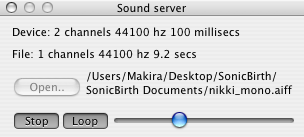
\includegraphics[width=3in]{../Artwork/sound_window.jpg}
\caption{The sound window}
\finf

This panel displays information on the current output device, current loaded file, and audio processing state. For the device, it shows the number of channels, the sample rate and the latency. The latency by default is set to 100ms. \footnote{The default latency is deliberately high: SonicBirth is not intended to be used as an audio processing application, but really just an AudioUnit design application. } 

Even if no sound is loaded, you can still press play. If your circuit has any inputs, it will receive silence. You can load a sound in AIFF or WAV format, and use it to test your circuit. Check section \ref{loading_a_sound} for more details.

\subsection{MIDI}

\debf
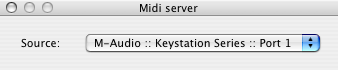
\includegraphics[width=3in]{../Artwork/midi_window.jpg}
\caption{The MIDI window}
\finf

This panel allows you to select which MIDI source is used to send MIDI events to the MIDI arguments of your circuits. This list will be updated when a source is added or removed while SonicBirth is running.

\subsection{Settings}

\debf
\includegraphics[width=3in]{../Artwork/settings_window.jpg}
\caption{The settings window for the look ahead element}
\finf

The settings panel shows specific informations about the currently selected element, or the displayed circuit if no element is selected. More details about these settings are given in the next section for the important elements. Most elements don't have any settings.

\subsection{Information}

\debf
\includegraphics[width=3in]{../Artwork/information_window.jpg}
\caption{The information window for the parametric EQ element}
\finf

The information panel displays useful information about either the selected element or the circuit (if no element is selected). Think of it as an inline help.

%-----------------------------------------------------------------------------------------------------------
\newpage
\section{Important elements}

This section gives more in-depth information about important elements you will use while designing an AudioUnit.

\subsection{Circuits}

\subsubsection{Root circuit}

This is the element that is at the base of your plugin model. This is what is seen by the host. There is always one and only one element of this kind, at level 0. It is also the element with the most settings:

\begin{itemize}

\item Name:  This is the name of the circuit as it will appear on disk and in the plugin host. It is limited in length (128 characters) and you cannot use special characters in it.

\item Author: This is an optional field where you can write the author's name. Useful if you intend to share your model file.

\item Company:  This is the company name that will appear in the generic graphical interface, and anywhere the host may use it.

\item Description: Here you should give a short description of your plugin, though most (all?) hosts ignore this information.

\item Subtype: This should be a unique four characters identifier. This comes from the way AudioUnits are listed by the operating system. You can use upper and lower case letters, numbers and most punctuation marks. Subtypes beginning by a capital 'S' are reserved for prebuilt plugins.

\item Inputs: Here you can enter the number of inputs your plugin will have.

\item Outputs: Here you can enter the number of outputs your plugin will have. A special case is when both the input and output count as one. In this case, the plugin will duplicate your circuit as needed, that is, you will be able to use it in an n to n (2/2, 3/3, 4/4, ...) configuration in your host.

\item Latency: This is used by the host to compensate for any latency in the circuit (delay line, lookahead, etc). This should be as precise as possible. If you are making an AudioUnit where the delay is intended, leave this to zero, since you do not want the host to compensate for it. The total latency given to the host will be the sum of the latency in milliseconds and the latency in samples (converted at runtime to milliseconds, depending on sample rate).

\item Tailtime: This is also used by the host to know how long your plugin can generate sound once its inputs have been silenced. You can use a conservative (but not extreme) value, it needs not be precise. For example, in a reverb circuit you might set this to 2000 or 3000 ms.

\item Comments: Like the author field, this is optional, and should mainly be used in case of redistribution, or as a small note pad.

\item Circuit min. size: This specifies the size under which scrollbars will appears in the circuit window. Should normally be set to a size where the circuit would be incorrectly displayed if the window is smaller.

\item Tempo and beat: The root circuit option, if enabled, will add two inputs to the root circuit, tempo and beat. This information is given by the host, if supported. Otherwise those inputs will be 0.

\item Sidechain: Some hosts support AudioUnits with multiple busses. SonicBirth can make plugins with 2 busses: the main one, and a sidechain one. Considering some hosts may not support sidechains, you should add a toggle to use or not the sidechain, if possible.

\item Arguments: You can specify the order in which the arguments will show up in the generic view in the host. Even if you use a custom gui, you should take a few seconds to reorder your arguments in case the host does not support custom gui.

\item Presets: If you want to include presets with your plugins, you can specify them. Clicking create will take a snapshot of the arguments current values and store them. You can then specify the name for the preset you create. As with the arguments, you can specify the order in which they appear. By clicking set,  the preset will be applied to the circuit, restoring the saved values.

\item Custom gui button and size: By enabling the custom gui button, you will be able to specify your own gui, using a background picture (or not) and by placing the argument in the gui design mode, then testing it in the runtime mode.

\item Front, contour and back colors: Even if you do not want to make a custom gui, you can change the colors of the arguments to something that suits you better.

\end{itemize}

\subsubsection{Subcircuit}

A subcircuit is a circuit which can be inserted in another one. It might be useful to group several elements in a logical group. It is also a way to hide arguments from the host. You can specify a few comments on a subcircuit explaining what it contains, if you want. It makes it easier to reuse.

\subsubsection{Piecewise circuit}

This is a complex circuit to answer a problem. Is is best explained by an example. Let's say you have a circuit, where you want the type of filter applied, lowpass or highpass, to be user selectable by an indexed argument. You could calculate both then use a comparator to select the value that will be used depending on the argument. But by doing so, you will calculate the value of the other filter for nothing, especially since the filter type will not be changed often (compared to the sample rate of the audio).

The answer is to create a piecewise circuit, which has a range input. In its settings window, you can specify many ranges. For each of them is associated a subcircuit. When you click {\em Next} on the document window, it will enter the currently selected range.

The number of inputs and outputs the subcircuit will have can be specified in the piecewise circuit window. For our example, a range would be created for the lowpass and one for the highpass, then you would enter each subcircuit/range to configure it.

The main difference with the comparator solution is the correct filter is selected one time by rendering cycle (typically a few milliseconds) and the other is not calculated.

\subsection{Internal arguments}

Some elements are automatically inserted in your root circuit depending on its content. You cannot delete or insert these elements yourself.

\subsubsection{Bit precision}

Your root circuit will always contain an element of type {\em Bit precision}. This is used to set the current precision of the rendering engine.

\subsubsection{Interpolation precision}

If any of the elements in the root circuit, or any subcircuits, interpolates the data, this element will appear.  There are two modes: no interpolation and linear interpolation. Using no interpolation is faster, but may have a lower quality sound. Using linear interpolation will sound better but will use more cpu. Depending on the amount of interpolation done, and the number of elements you use that interpolate, the difference in speed can vary.

\subsubsection{Midi settings}

If you use any MIDI arguments, this element will be automatically added to your root circuit. Instead of having a channel and controller parameter for each one of your midi arguments, these settings are controlled by this central element. 

\subsection{Arguments}

The arguments are the elements that will appear as parameters in your final plugin.  There are three types of basic elements, with more to come for future releases. Every argument has name that can be user specified, and a realtime switch which tells the host if the associated parameters should be changed while playing audio or not (some hosts may completely ignore this).

\subsubsection{Boolean}

A boolean argument is an on/off switch. 

\debf
\includegraphics[width=1.2in]{../Artwork/boolean.jpg}
\caption{The boolean argument}
\finf

For both states, you can specify the value it will output. You can change its state directly by clicking on the drawn switch. The other argument can be controlled in the same way.

\subsubsection{Indexed}

An indexed argument is a popup menu with different choices. 

\debf
\includegraphics[width=2in]{../Artwork/indexed.jpg}
\caption{The indexed argument}
\finf

You can specify these choices by creating, deleting and ordering the items using the settings window. For each item, any value can be given. This value will be outputted when the item is selected.

\subsubsection{Slider}

A slider argument is a variable value with a maximum and a minimum. 

\debf
\includegraphics[width=1.2in]{../Artwork/slider.jpg}
\caption{The slider argument}
\finf

It will appear as a slider in a generic view and as a circular knob in a custom view (in the host that loads the plugin). The {\em Show value} button, when selected, will make the current value appear under the knob.

The {\em Type} attribute is a hint for the host so it can know what type of value the slider is representing. It is optional and will only be showed in a generic gui. For a slider controller gain, you should specify if the value is in linear units of decibels.

The {\em Mapping} attribute can be either linear or logarithmic. If you have a slider with minimum 20 and maximum 20000 (a frequency range), in linear mapping, the middle value would be around 10000, and in logarithmic mapping it would be around 450.

\subsubsection{Points}

An element allowing you to draw a line, with either step, linear or spline interpolation. Used to drive other elements. This argument will not appear in the generic view of exported plugins, therefore in order to be usable you will have to build a custom gui for your plugin. Internally the points are represented in a 1 by 1 box, with the lower left corner at position (0,0) and upper right corner at position (1,1). The {\em Points apply} element can translate and scale this box. Other elements may use this information differently.

\subsubsection{Points Envelope}

A variation on the {\em Points} element where attack, sustain and release have different sections.

\subsubsection{Points Frequency}

A variation on the {\em Points} element with markers for frequency, as used by the {\em Points To FFT} and {\em FFT generator}�elements.

\subsubsection{XY Pad}

This a basically two sliders represented together by a box and a point. One slider takes its value by the horizontal position of the point while the other checks the vertical position.
 
 \subsubsection{Audiofile argument}

Allows the user to load an audio file. The number of outputs is decided at design time. If the loaded file has too many channels, the extra ones are ignored. If it does not have enough, the extra outputs will have empty sound (silence). In case of a single channel loaded in a multiple output configuration, the channel will be given on all outputs.

\subsection{Midi arguments}

MIDI input is supported by the use of MIDI arguments. These arguments will receive MIDI events and change their output accordingly.

\subsubsection{Midi slider}

The {\em Midi slider} is the same as a normal slider, except it can also be controlled by midi events. To easily find which controller should be used, you can set it to learn. It will then set the controller attribute to the first controller event it receives. If you have multiple MIDI sliders, do not set them all to learn by default, since they will all switch to it simultaneously when they receive the first controller event... unless you want it like that. For example, a multiband equalizer could have some bands attached to the same controller instead of individually.

\subsubsection{Midi mono note}

The {\em Midi mono note} element outputs the last note that was pressed, with its velocity. If multiple note are pressed, it will output the last one pressed, and if the note is depressed, it will output the previous note. When no note is pressed, the specified default values are outputted. If the {\em Hold note} button is selected, it will not revert to the default value when the last note is depressed but rather hold it.

\subsubsection{Midi multi note}

Like the piecewise circuit element the {\em Midi multi note} is a complex element to answer a problem. If you have a sine generator and want to be able to have more than one note played simultaneously, you have to duplicate the sine generator for each additional note pressed. This is exactly what {\em Midi multi note} does. It contains a subcircuit which you can edit, and this circuit is duplicated on the fly for each note pressed. The output of each currently active subcircuit is summed and then outputted as one output.

\subsubsection{Midi multi note env}

This is a variation of  {\em Midi multi note}, where the envelope is specified visually, through a {\em Points Envelope} argument.

\subsection{FFT elements}

Coming soon \ldots Until then, you can take a look at the graphic equalizer plugin.


%-----------------------------------------------------------------------------------------------------------
\newpage
\section{Circuit examples}

\subsubsection{The simplest circuit: passthrough}

\debf
\includegraphics[width=3in]{../Artwork/passthrough.jpg}
\caption{A passthrough circuit}
\finf

This is the first thing you should try. The detailed steps to follow are:

\begin{enumerate}

\item Click on the background to select the root circuit.
\item In the settings window, specify one input and one output.
\item Drag a link between the input to the output.
\item Use the sound panel to load a sound.
\item Click play.

\end{enumerate}

You should now hear the sound you just loaded.

\subsubsection{Stereo to mono}

\debf
\includegraphics[width=3in]{../Artwork/stereo_to_mono.jpg}
\caption{A stereo to mono circuit}
\finf

Once you made the passthrough circuit, try this:

\begin{enumerate}

\item Click on the background to select the root circuit.
\item In the settings window, specify two inputs.
\item Use the {\em Insert element...} popup menu to insert an {\em Addition} element, from the {\em Algebraic} category.
\item Connect both inputs of the circuit to the inputs of the addition element.
\item Connect the output of the addition element to the output of the circuit.
\item Make sure the loaded sound is actually stereo. If not load another sound.
\item Click play.

\end{enumerate}

You should hear the mono summation of your original file. By the way, you can do all these modifications while the circuit is playing.

\subsubsection{A multiband reverb}

From now on, only the general steps will be given, so you should understand the basics when trying this.

\debf
\includegraphics[width=4in]{../Artwork/multiband_freeverb.jpg}
\caption{A multiband reverb circuit}
\finf

\begin{enumerate}

\item Create a two input, two output root circuit.
\item Insert two crossover elements, one for each channel.
\item Use the same frequency configured slider for both.
\item Insert two freeverb elements.
\item Connect the two high outputs of both crossovers to one freeverb element.
\item Same for the low outputs.
\item Now it is up to you to decide if you want to double every settings for the freeverb, or if you want some to be in common. For exemple, the wet and dry settings could be shared. With one of the freeverb elements selected, read from the information window what parameters and range are expected for this element.
\item Insert two addition elements.
\item Connect the left outputs of both freeverb elements to one addition.
\item Same for the right outputs.
\item Connect the outputs of the addition elements to the output of the circuit.
\item Test it.

\end{enumerate}

There is an infinite variation for this. You could add a highpass after the reverbing elements to cut the rumbles. You could have some sliders as MIDI sliders instead. You could add feedback loops to add extra reverberation. Or a valve element to add some distortion in the path. Or an atan element to slightly compress the signal. Or use an envelope follower on the input signal to control the room size of the freeverb element. As you see, it can get as complicated as you want. For very big circuits, you will want to try the mini mode.

\subsubsection{A software synth}

A software synth is usually splitted in two stages, the sound generation, and the sound processing. The sound generation will be done inside a MIDI multi note element. The sound processing is done after. As for the multiband reverb, the steps presented here are general.

\debf
\includegraphics[width=4in]{../Artwork/midi_multi_note.jpg}
\caption{Inside multi midi note}
\finf

\debf
\includegraphics[width=4in]{../Artwork/rainy_synth.jpg}
\caption{A rainy software synth}
\finf

\begin{enumerate}

\item Create a zero input, one output root circuit.
\item Insert a MIDI multi note element.
\item Give it one output.
\item Insert and connect a slider to the its attack input.
\item Insert and connect a slider to the its release input.
\item Go inside it by clicking the {\em Next} button while it is selected.
\item There will be two inputs available: the frequency and velocity.
\item Insert a sine generator.
\item Connect the frequency input to the sine generator frequency input.
\item Insert a multiplication element.
\item Connect the velocity input and the output of the sine generator to the inputs of the multiplication element.
\item Connect the output of the multiplication element to the output of the subcircuit.
\item Click {\em Prev} to return to the root circuit.
\item Insert a bandstop element (we'll use it in an abnormal way to add some distortion and stereo width).
\item Insert a linear noise generator
\item Insert an absolute
\item Insert a multiplication and a constant.
\item Set the constant to 20000.
\item Connect the output of the MIDI multi note to the other input of the bandstop.
\item Connect the output of the noise generator to the absolute element.
\item Connect the output of the constant and the absolute element to the multiplication element.
\item Connect the output of the multiplication unit to one frequency input of the bandstop.
\item Repeat for the other frequency input.
\item Connect the output of the bandstop to the output of the root circuit.
\item Press a note and hear a rainy sine sound.

\end{enumerate}

If you want to pass arguments to the element inside the MIDI multi note, simply give it some inputs and connect the arguments to them. You can only connect the outputs of an argument to the inputs of another argument.

%-----------------------------------------------------------------------------------------------------------
\newpage
\section{Custom gui}

A great sounding plugin is very good, but with a nice looking gui, it is even better! That is why SonicBirth allows you to make a custom gui. 

\debf
\includegraphics[width=4in]{../Artwork/custom_gui.jpg}
\caption{Custom gui settings}
\finf

\subsection{Designing the interface}

The first step to take is activating the {\em Custom gui} button on the settings window of the root circuit, then switch to gui design mode. Set a suitable size. Bear in mind that not everyone has a very high resolution monitor, so keep it small if you plan on sharing it.

\subsubsection{Placing the elements}

The next step is to place the arguments. Simply drag \& drop them where you want them to appear. Simple as that. But do not make them overlap.

\subsubsection{Selecting the colors}

The arguments are drawn with three selectable colors. These colors can be set below 100\% opaque. In fact, you can set the opaque value to 0\% for both the background and contour colors and use the background image instead.

\subsubsection{Loading a background picture}

The arguments will not display any labels such as minimum and maximum value, or the argument name. These are expected to be done in the background image. One trick is to take a screenshot of the window when the arguments are placed (using Command-Shift-3), then load this as the starting point in your graphical application. Save it as either jpg, gif, png or tiff format. ({\it Since the image file will be included as it is on disk in the circuit model file, using jpg is strongly suggested as it will keep the size smaller})

Back in SonicBirth, click load, select your background picture, and you are done!

\subsection{Testing the interface}

In the runtime mode, you can test your interface as it will behave in the host. Not much to say.

%-----------------------------------------------------------------------------------------------------------
% The following is auto-generated.
%150 elements
\newpage
\section{List of elements}
\subsection{Algebraic}
\subsubsection{Addition}
Outputs the sum of both inputs.

Inputs : a, b.

Outputs : a+b.

\subsubsection{Add Many}
Outputs the summation of 3 to 16 inputs.

Inputs : in0, in1, in2, in3.

Outputs : out.

\subsubsection{Substraction}
Outputs (a - b).

Inputs : a, b.

Outputs : a-b.

\subsubsection{Multiplication}
Outputs (a * b).

Inputs : a, b.

Outputs : a*b.

\subsubsection{Division}
Outputs (a / b).

Inputs : a, b.

Outputs : a/b.

\subsubsection{Constant Addition}
Adds a constant number.

Inputs : i.

Outputs : o.

\subsubsection{Constant Substraction}
Substracts a constant number.

Inputs : i.

Outputs : o.

\subsubsection{Constant Multiplication}
Multiply by a constant number.

Inputs : i.

Outputs : o.

\subsubsection{Constant Division}
Divides by a constant number.

Inputs : i.

Outputs : o.

\subsubsection{Constant Substraction Alt.}
Constant number substracted by input.

Inputs : i.

Outputs : o.

\subsubsection{Constant Division Alt.}
Constant number divided by input.

Inputs : i.

Outputs : o.

\subsubsection{Negation}
Outputs -x.

Inputs : x.

Outputs : -x.

\subsubsection{Inverse}
Outputs 1/x.

Inputs : x.

Outputs : 1/x.

\subsubsection{Absolute}
Outputs |x| (x if x>=0, -x if x<0).

Inputs : x.

Outputs : |x|.

\subsubsection{Absolute/Sign}
Outputs |x| (x if x>=0, -x if x<0), and sign of x (1 for pos, -1 for neg).

Inputs : x.

Outputs : |x|, sign.

\subsubsection{Direction}
Outputs 1 if input is augmenting, -1 if it is descending, 0 otherwise.

Inputs : x.

Outputs : dir.

\subsubsection{Multiply-Add}
Outputs (a*b)+c.

Inputs : a, b, c.

Outputs : (a*b)+c.

\subsubsection{Multiply-Sub}
Outputs (a*b)-c.

Inputs : a, b, c.

Outputs : (a*b)-c.

\subsubsection{Neg. Multiply-Add}
Outputs -((a*b)+c).

Inputs : a, b, c.

Outputs : -((a*b)+c).

\subsubsection{Neg. Multiply-Sub}
Outputs -((a*b)-c).

Inputs : a, b, c.

Outputs : -((a*b)-c).

\subsection{Function}
\subsubsection{Modulus}
Outputs x \% y (x mod y).

Inputs : x, y.

Outputs : x\%y.

\subsubsection{Ceil}
Rounds to smallest integral value not less than x.

Inputs : x.

Outputs : o.

\subsubsection{Floor}
Rounds to largest integral value not greater than x.

Inputs : x.

Outputs : o.

\subsubsection{Nearest integer}
Rounds to nearest integer.

Inputs : x.

Outputs : o.

\subsubsection{Exponential}
Outputs e\^x.

Inputs : x.

Outputs : e\^x.

\subsubsection{Natural logarithm}
Outputs ln(x).

Inputs : x.

Outputs : ln(x).

\subsubsection{Logarithm base 10}
Outputs log10(x).

Inputs : x.

Outputs : log10(x).

\subsubsection{Power}
Outputs x\^y.

Inputs : x, y.

Outputs : x\^y.

\subsubsection{Square root}
Outputs sqrt(x).

Inputs : x.

Outputs : sqrt(x).

\subsubsection{Reverse square root}
Outputs rsqrt(x).

Inputs : x.

Outputs : rsqrt(x).

\subsubsection{Quadratic Bezier}
Outputs (1-t)\^2*a + 2*t*(1-t)*b + t\^2*c, where t is clamped to 0 .. 1. See http://en.wikipedia.org/wiki/B\%e9zier\_curve.

Inputs : t, a, b, c.

Outputs : o.

\subsection{Trigonometric}
\subsubsection{Sinus}
Outputs the sinus of the input.

Inputs : x.

Outputs : sin x.

\subsubsection{Cosinus}
Outputs the cosinus of the input.

Inputs : x.

Outputs : cos x.

\subsubsection{Tangent}
Outputs the tangent of the input.

Inputs : x.

Outputs : tan x.

\subsubsection{Sinus and cosinus}
Outputs both the sinus and the cosinus of the input.

Inputs : x.

Outputs : sin x, cos x.

\subsubsection{Hyperbolic sinus}
Outputs the hyperbolic sinus of the input.

Inputs : x.

Outputs : sinh x.

\subsubsection{Hyperbolic cosinus}
Outputs the hyperbolic cosinus of the input.

Inputs : x.

Outputs : cosh x.

\subsubsection{Hyperbolic tangent}
Outputs the hyperbolic tangent of the input.

Inputs : x.

Outputs : tanh x.

\subsubsection{Arc sinus}
Outputs the arc sinus of the input.

Inputs : x.

Outputs : asin x.

\subsubsection{Arc cosinus}
Outputs the arc cosinus of the input.

Inputs : x.

Outputs : acos x.

\subsubsection{Arc tangent}
Outputs the arc tangent of the input.

Inputs : x.

Outputs : atan x.

\subsubsection{Arc tangent (x, y)}
Outputs the arc tangent of y/x.

Inputs : x, y.

Outputs : atan(y/x).

\subsubsection{Inverse hyperbolic sinus}
Outputs the inverse hyperbolic sinus of the input.

Inputs : x.

Outputs : asinh x.

\subsubsection{Inverse hyperbolic cosinus}
Outputs the inverse hyperbolic cosinus of the input.

Inputs : x.

Outputs : acosh x.

\subsubsection{Inverse hyperbolic tangent}
Outputs the inverse hyperbolic tangent of the input.

Inputs : x.

Outputs : atanh x.

\subsection{Arguments }
\subsubsection{Boolean}
Boolean button with value for true and for false.

Outputs : value.

\subsubsection{Slider}
Basic slider with min/max.

Outputs : value.

\subsubsection{Indexed}
Indexed popup button with multiple values.

Outputs : value.

\subsubsection{Points}
Set of points making a line. Double-click to insert a point. Use left and right arrow to change interpolation type. Delete key to remove a point.

Outputs : pts.

\subsubsection{Points Envelope}
Set of points defining attack, loop and release.  Double-click to insert a point. Use left and right arrow to change interpolation type. Delete key to remove a point.

Outputs : pts.

\subsubsection{Points Frequency}
Set of points suitable for fft conversion or generation.  Double-click to insert a point. Use left and right arrow to change interpolation type. Delete key to remove a point.

Outputs : pts.

\subsubsection{XY Pad}
Two sliders combined in a XY pad.

Outputs : x, y.

\subsubsection{Audio file argument}
User selectable audio file with preset channel count.

Outputs : chan 0.

\subsubsection{Keyboard Tap}
Emits a single 1 when receiving a key stroke.

Outputs : tap.

\subsection{Midi arguments}
\subsubsection{Midi slider}
Outputs the value of the a midi parameter in a user supplied range.

Outputs : value.

\subsubsection{Midi note state}
Outputs the state (pressed or not) and velocity (0 to 1) for each specified note.

\subsubsection{Midi mono note}
Outputs the note and velocity (in the range 0 - 1) of the current presser note. You can select to hold the last note pressed.

Outputs : note, velo, numb.

\subsubsection{Midi multi note}
Duplicates the subcircuit on the fly for each pressed note, up to a maximum of 16. The outputs of these subcircuits are summed, then outputed. You can specify the attack and release time in milliseconds. Both are clamped to 0 .. 60000 milliseconds. You must stop/start for changes to take effect.

Inputs : atck, rlse.

\subsubsection{Midi multi note envelope}
Duplicates the subcircuit on the fly for each pressed note, up to a maximum of 16. The outputs of these subcircuits are summed, then outputed. You can specify the attack, loop and release time in milliseconds. All are clamped to 0 .. 60000 milliseconds. You must stop/start for changes to take effect.

Inputs : atck, loop, rlse, pts.

\subsubsection{Midi XY Pad}
Two sliders combined in a XY pad, midi controllable. (Y controller is always the one following the X controller).

Outputs : x, y.

\subsection{Display}
\subsubsection{Display value}
Shows the first value of the input of each audio cycle. Can be used in the plugin interface.

Inputs : in.

\subsubsection{Display Osc.}
An oscilloscope that can be used in the plugin interface.

Inputs : in.

\subsubsection{Display Osc. (Var. res.)}
An oscilloscope that can be used in the plugin interface.

Inputs : in, res.

\subsubsection{Display Meter}
A value meter that can be used in the plugin interface.

Inputs : in.

\subsection{Analysis}
\subsubsection{Envelope Follower}
Envelope follower with variable attack and release time, in milliseconds. The output is in positive linear units.

Inputs : in, atck, rlse.

Outputs : env.

\subsubsection{Look ahead}
Basic look ahead: outputs the current enveloppe of the input signal, and the delayed signal.

Inputs : in.

Outputs : out, env.

\subsubsection{BPM Counter}
BPM counter analyses its input and outputs the current bpm. Uses the last 4 events to average the bpm. Is considred an event when its input passes from under or equal to 0.5 to over 0.5.

Inputs : in.

Outputs : bpm.

\subsubsection{Debug}
Shows the first value of the input of each audio cycle.

Inputs : in.

\subsubsection{Debug Osc.}
An oscilloscope for debugging purpose.

Inputs : in.

\subsection{Comparators}
\subsubsection{Minimum}
Outputs the smallest of both inputs.

Inputs : a, b.

Outputs : min(a,b).

\subsubsection{Maximum}
Outputs the largest of both inputs.

Inputs : a, b.

Outputs : max(a,b).

\subsubsection{Sort}
Outputs the min and max of both inputs.

Inputs : a, b.

Outputs : min, max.

\subsubsection{Less}
If (a < b) the outputs c else outputs d.

Inputs : a, b, c, d.

Outputs : o.

\subsubsection{Equal}
If (a = b) the outputs c else outputs d.

Inputs : a, b, c, d.

Outputs : o.

\subsubsection{Greater}
If (a > b) the outputs c else outputs d.

Inputs : a, b, c, d.

Outputs : o.

\subsection{Converters}
\subsubsection{Msec to samples}
Converts milliseconds into samples.

Inputs : ms.

Outputs : smpl.

\subsubsection{Samples to msec}
Converts samples into milliseconds.

Inputs : smpl.

Outputs : ms.

\subsubsection{Linear to db}
Converts linear values into decibels.

Inputs : lin.

Outputs : db.

\subsubsection{Db to linear}
Converts decibels into linear values.

Inputs : db.

Outputs : lin.

\subsection{Delays}
\subsubsection{Delay}
Delays the input signal by a variable time (maximum is user specified - clamped to 60 seconds). The dly input is in seconds.

Inputs : in, dly.

Outputs : out.

\subsubsection{Delay (samples)}
Delays the input signal by a variable time in samples (max: 100000).

Inputs : in, dly.

Outputs : out.

\subsubsection{Delay Sinc (samples)}
Delays the input signal by a variable time in samples, using 16 points Blackman windowed sinc interpolation (min delay: 8 samples, max delay: 100000 samples).

Inputs : in, dly.

Outputs : out.

\subsection{Generators}
\subsubsection{Sine Wave}
Generates a sine wave, of frequency f (hz) and phase p (0 to 2pi).

Inputs : f, p.

Outputs : tone.

\subsubsection{Fast Sine Wave}
Generates a sine wave, of frequency f (hz). Low cpu usage.

Inputs : f.

Outputs : tone.

\subsubsection{Saw Wave}
Generates a saw wave, of frequency f (hz) and phase p (0 to 2pi).

Inputs : f, p.

Outputs : sawave.

\subsubsection{Triangle Wave}
Generates a triangle wave, of frequency f (hz) and phase p (0 to 2pi).

Inputs : f, p.

Outputs : twave.

\subsubsection{Square wave}
Generates a square wave, of frequency f (hz) and phase p (0 to 2pi).

Inputs : f, p.

Outputs : swave.

\subsubsection{Linear Noise}
Generates linear noise (random values between -1 and 1).

Outputs : lnoise.

\subsubsection{White Noise}
Generates white noise (random values between -1 and 1, with gaussian distribution).

Outputs : wnoise.

\subsubsection{Pink Noise}
Generates pink noise (1/f noise).

Outputs : pnoise.

\subsubsection{Random}
Generates random values between -1 and 1, changing the value at frequency f.

Inputs : f.

Outputs : rnd.

\subsubsection{Random ramp}
Generates random values between -1 and 1, changing the value at frequency f, interpolating between values.

Inputs : f.

Outputs : rnd.

\subsubsection{FFT Generator}
Generates waves using FFT based on input points..

Inputs : pts.

Outputs : snd.

\subsection{Filters}
\subsubsection{DC Blocker}
Cuts frequencies below 20 hz.

Inputs : in.

Outputs : out.

\subsubsection{Parametric Eq.}
Parametric Eq: f is the center frequency, g is the gain or cut in dB (clamped in the range -15 .. 15). Q should be between 0.3 and 15.

Inputs : in, f, g, Q.

Outputs : out.

\subsubsection{Peak}
Peaking eq, with constant Q (10) and dB gain (20 dB).

Inputs : in, f.

Outputs : out.

\subsubsection{Notch}
Notch with constant bandwitdh (0.1 octave).

Inputs : in, f.

Outputs : out.

\subsubsection{Lowpass}
Lowpass filter, 12/db octave (Butterworth), with variable cutoff frequency (clamped to [1, 20000]).

Inputs : in, f.

Outputs : out.

\subsubsection{Highpass}
Highpass filter, 12/db octave (Butterworth), with variable cutoff frequency (clamped to [1, 20000]).

Inputs : in, f.

Outputs : out.

\subsubsection{Resonant lowpass}
Resonant lowpass filter, 12/db octave (Butterworth), with variable cutoff frequency (clamped to [20, 20000]). Resonance should be between sqrt(2), that is 1.414..., for no resonance, and 0.1 for max resonance.

Inputs : in, f, r.

Outputs : out.

\subsubsection{Resonant highpass}
Resonant highpass filter, 12/db octave (Butterworth), with variable cutoff frequency (clamped to [20, 20000]). Resonance should be between sqrt(2), that is 1.414..., for no resonance, and 0.1 for max resonance.

Inputs : in, f, r.

Outputs : out.

\subsubsection{Crossover}
Linkwitz-Riley 24db/octave crossover.

Inputs : in, f.

Outputs : high, low.

\subsubsection{Bandstop}
24db/octave bandstop.

Inputs : in, f1, f2.

Outputs : out.

\subsubsection{Bandpass}
24db/octave bandpass.

Inputs : in, f1, f2.

Outputs : out.

\subsubsection{Lowpass (fast)}
Same as lowpass, but only checks its parameter once per audio cycle.

Inputs : in, f.

Outputs : out.

\subsubsection{Highpass (fast)}
Same as highpass, but only checks its parameter once per audio cycle.

Inputs : in, f.

Outputs : out.

\subsubsection{Resonant lowpass (fast)}
Same as resonant lowpass, but only checks its parameters once per audio cycle.

Inputs : in, f, r.

Outputs : out.

\subsubsection{Resonant highpass (fast)}
Same as resonant highpass, but only checks its parameters once per audio cycle.

Inputs : in, f, r.

Outputs : out.

\subsubsection{Crossover (fast)}
Same as crossover, but only checks its parameter once per audio cycle.

Inputs : in, f.

Outputs : high, low.

\subsubsection{Bandstop (fast)}
Same as bandstop, but only checks its parameters once per audio cycle.

Inputs : in, f1, f2.

Outputs : out.

\subsubsection{Bandpass (fast)}
Same as bandpass, but only checks its parameters once per audio cycle.

Inputs : in, f1, f2.

Outputs : out.

\subsubsection{Allpass}
Allpass, with variable delay, clamped between 0 and 1 sec. Equivalent to a feedback comb filter followed by a feedforward comb filter. y(t) = a*x(t) + x(t-dly) - b*y(t-dly)

Inputs : in, a, b, dly.

Outputs : out.

\subsubsection{Feedback Comb}
Feedback comb, with variable delay, clamped between 0 and 1 sec. y(t) = a*x(t) - b*y(t-dly)

Inputs : in, a, b, dly.

Outputs : out.

\subsubsection{Feedforward Comb}
Feedforward comb, with variable delay, clamped between 0 and 1 sec. y(t) = a*x(t) + b*x(t-dly)

Inputs : in, a, b, dly.

Outputs : out.

\subsubsection{Formant filter}
Formant filter with variable phonemes. Choose one on v1, another on v2, and you can mix between the two using input m [0,1]. Here are the phonemes:
phoneme 0: eee (beet)
phoneme 1: ihh (bit)
phoneme 2: ehh (bet)
phoneme 3: aaa (bat)
phoneme 4: ahh (father)
phoneme 5: aww (bought)
phoneme 6: uhh (but)
phoneme 7: uuu (foot)
phoneme 8: ooo (boot)
phoneme 9: rrr (bird)
phoneme 10: lll (lull)
phoneme 11: mmm (mom)
phoneme 12: nnn (nun)


Inputs : i, v1, v2, m.

Outputs : o.

\subsection{Feedback}
\subsubsection{Feedback}
Allows a feedback loop, with fixed delay (0.010000 seconds).

Inputs : in.

Outputs : out.

\subsection{Distortion}
\subsubsection{Valve}
Valve distortion simulation. Level and character range is 0 to 1. Level is how much the signal is driven against the limit of the valve. Character is the hardness of the sound.

Inputs : in, lv, ch.

Outputs : out.

\subsubsection{Scraper}
Degrades quality of sampling rate, and bit depth (parameters in the range [0, 1], where 0 is lowest quality and 1 is original signal).

Inputs : in, sr, bd.

Outputs : out.

\subsubsection{Scraper (quick)}
Degrades quality of sampling rate, and bit depth (parameters in the range [0, 1], where 0 is lowest quality and 1 is original signal). Less precise but faster version.

Inputs : in, sr, bd.

Outputs : out.

\subsection{Audio file}
\subsubsection{Audio file}
Loads an audio file and outputs each channel.

\subsubsection{Audio player}
Audio player plays the audio from the buffer when trig is non-zero. Start and end represents the playing offset. If end is smaller than start, speed is negated. Both these values should be between 0 and 1. Playing will loop if the loop input is non-zero. Speed give the playing speed, should be between -5 and 5. A negative speed means the buffers is played reversed.

Inputs : trig, start, end, loop, speed, buf.

Outputs : o.

\subsection{FFT}
\subsubsection{FFT Sync}
States the fft size and block positions.

Outputs : sync.

\subsubsection{Forward FFT}
Outputs the forward fft of the input, with variable block size (delay).

Inputs : sync, in.

Outputs : real, imag.

\subsubsection{Inverse FFT}
Outputs the inverse fft of the input.

Inputs : sync, real, imag.

Outputs : out.

\subsubsection{Complex to Polar}
Converts complex fft blocks into polar fft blocks.

Inputs : sync, real, imag.

Outputs : ampl, phas.

\subsubsection{Polar to Complex}
Converts polar fft blocks into complex fft blocks.

Inputs : sync, ampl, phas.

Outputs : real, imag.

\subsubsection{Convolve}
Convolve two fft signals (in the complex plane).

Inputs : sync, r1, i1, r2, i2.

Outputs : ro, io.

\subsubsection{Points To FFT}
Transforms a points function into frequency amplitudes. Range is in db.

Inputs : sync, pts, range.

Outputs : real, imag.

\subsubsection{Audio file To FFT}
Transforms an audio file to an fft block (considering samples up to half the fft block size).

Inputs : sync, af.

Outputs : real, imag.

\subsection{Miscellaneous}
\subsubsection{Circuit}
A circuit inside another.

\subsubsection{Constant}
A constant number.

Outputs : o.

\subsubsection{Equation}
A mathematical equation. You can use these functions:

sin(x), cos(x), tan(x), asin(x), acos(x), atan(x),
sinh(x), cosh(x), tanh(x), asinh(x), acosh(x), atanh(x),
atan2(x,y), pow(x,y), min(x,y), max(x,y), mod(x,y),
abs(x), floor(x), ceil(x), nearint(x), inv(x),
exp(x), log(x), log10(x), sqrt(x), revsqrt(x).

Speed: compare the execute plan for:
	- i0*2*3 and i0*(2*3)
	- i0*i0*i0*i0 and (i0*i0)*(i0*i0)

You can also enter an equation in the constant element (sqrt(2) for example).

Inputs : i0.

Outputs : o.

\subsubsection{Piecewise circuit}
Depending on the value of the range input, a specific subcircuit is executed. This value is checked once per block of samples. The subcircuit which is entered when clicking next depends on the selected row in the settings window.

Inputs : range.

\subsubsection{Samplerate Doubler}
Audio processing inside this circuit is done at double sample rate, which can be useful (sounds better) for some type of calculations (filters).

\subsubsection{Timer}
Outputs the time in seconds, when run is 1, outputs 0 otherwise. Time is reset then run switchs to 1.

Inputs : run.

Outputs : time.

\subsubsection{Timer loop}
Outputs the time in seconds, looping back to 0 when arriving to the max time specified. Loops back to 0 when arriving to the max time specified.If the max is equal or smaller than 0, then it does not loop. Time is reset then run switchs to 1.

Inputs : run, max.

Outputs : time.

\subsubsection{Freeverb}
Jezar's freeverb. (Room size: 0.5 to 0.999, damp: 0 to 1, wet: 0 to 3, dry: 0 to 2, width: 0 to 1, freeze: 0/no or 1/yes)

Inputs : in1, in2, room size, damp, wet, dry, width, freeze.

Outputs : out1, out2.

\subsubsection{Cleaner}
Removes denormals, infinities and nan (not a number). Use this if your circuit can potentially create those numbers (division by 0, tan(pi/2), etc). The signal can optinnaly be clamped to [-1 .. 1].

Inputs : in.

Outputs : out.

\subsubsection{Points apply}
Applies the points function using x and y as origin, width and height as size.

Inputs : i, x, y, w, h, pts.

Outputs : o.

\subsubsection{Bufferizer}
Buffer object with three modes: silence (0), play (1), record (2). In playing mode, start and end represents the playing offset. If end is smaller than start, speed is negated. Both these values should be between 0 and 1. Playing will loop if the loop input is non-zero. Speed give the playing speed, should be between -5 and 5. A negative speed means the buffers is played reversed. In record mode, the buffer is filled from start up to its capacity.

Inputs : in, mode, start, end, loop, speed.

Outputs : out.

\subsubsection{Trigger}
Trigger sends either the on value or off value depending on its internal state. Its state is initialized as off. If the t (trigger) input is higher than the tt (trigger threshold) input, its state is turned on. If the r (reset) input is higher than the rt (reset threshold) input, its stated is turned off. In case both events are occuring simultaneously, the state is turned on.

Inputs : tt, rt, t, r, on, off.

Outputs : o.

\subsubsection{Change Slower}
Slows the rate of change of the input on a specified amount of milliseconds.

Inputs : i.

Outputs : o.

\subsubsection{Convolving reverb}
Convolving reverb, 4096 samples latency. Max reverb length: 2457600 samples. Memory usage at max reverb length: 75.4 MBs

Inputs : in, ir.

Outputs : out.

\subsubsection{AudioUnit}
Wraps a third party audiounit.

Inputs : tempo, beat.

\subsubsection{AudioUnit (midi)}
Wraps a third party audiounit.

Inputs : tempo, beat.

\subsubsection{Granulate effect}
Granulator effect. Delay is max delay in seconds to create grain from (max 10 seconds). DRandomness is a value between 0 and 1 affecting the grain's delay.Ramp is a value between 0 and 100. At 0 no attack or decay is used. At 100 it gives a triangular envelope, at 50 a trapezoidal envelope. Voices is the number of simultaneous grains (max 100). Length is the duration of grains in seconds (max 1 second). LRandomness is a value between 0 and 1 affecting the grain's length.Silence is the duration of silence between grains in seconds (max 10 seconds). SRandomness is a value between 0 and 1 affecting the silence's length.

Inputs : i, delay, drndness, ramp, voices, length, lrndness, silence, srndness.

Outputs : o.

\subsubsection{Granulate effect with pitch}
Granulator effect with variable picth. Delay is max delay in seconds to create grain from (max 10 seconds). DRandomness is a value between 0 and 1 affecting the grain's delay.Ramp is a value between 0 and 100. At 0 no attack or decay is used. At 100 it gives a triangular envelope, at 50 a trapezoidal envelope. Voices is the number of simultaneous grains (max 100). Length is the duration of grains in seconds (max 1 second). LRandomness is a value between 0 and 1 affecting the grain's length.Silence is the duration of silence between grains in seconds (max 10 seconds). SRandomness is a value between 0 and 1 affecting the silence's length.Pitch is the grain playing speed (0.5 to 5) - can be negative. PRandomness is a value between 0 and 1 affecting the pitch.

Inputs : i, delay, drndness, ramp, voices, length, lrndness, silence, srndness, pitch, prndness.

Outputs : o.

\subsection{Internal}
\subsubsection{Interpolation Precision}
Sets the interpolation type of the audio engine.

\subsubsection{Bit Precision}
Sets the bit precision of the audio engine.

\subsubsection{Midi settings}
MIDI settings central control.

\end{document}

